\chapter{力学：从最小作用量到牛顿定律}
\label{ch:mechanics}

\section{概述}
R2（$\delta S=0$）给定拉格朗日量 $L$，Euler-Lagrange 方程就产生全部经典力学运动方程。

\[
\text{R2: } \delta S = 0 \;\longrightarrow\; \text{Euler-Lagrange} \;\longrightarrow\; \text{牛顿三定律} \;\longrightarrow\; \text{引力 + Kepler}
\]

\section{Euler-Lagrange 方程}

\begin{lawbox}[Euler-Lagrange 方程]
\[
\frac{d}{dt}\!\left( \frac{\partial L}{\partial \dot{q}_i} \right) - \frac{\partial L}{\partial q_i} = 0
\]
\textbf{前提}：R2（$\delta S = 0$）
\end{lawbox}

\subsection{图示：变分法的几何意义}

\begin{center}
\begin{tikzpicture}[scale=1.3]
  \draw[->] (0,0) -- (4.5,0) node[right] {$t$};
  \draw[->] (0,0) -- (0,3.5) node[above] {$q$};
  \fill[red] (0.5,1.0) circle (2pt);
  \fill[red] (3.8,2.8) circle (2pt);
  \node[left] at (0.5,1.0) {$A$};
  \node[right] at (3.8,2.8) {$B$};
  % True path
  \draw[principleblue,very thick] plot[domain=0.5:3.8,samples=40] (\x, {1.0 + 0.5*(\x-0.5) + 0.15*(\x-0.5)^2});
  \node[principleblue] at (3.2,1.6) {真实路径 $q(t)$};
  % Varied path
  \draw[gray,dashed] plot[domain=0.5:3.8,samples=40] (\x, {1.0 + 0.3*(\x-0.5) + 0.3*(\x-0.5)^2 - 0.04*(\x-0.5)^3});
  \node[gray] at (2.8,2.5) {变分路径 $q(t)+\delta q$};
  % Labels
  \node at (2.2,-0.4) {$\delta S = 0$ 在真实路径上};
\end{tikzpicture}
\end{center}

真实路径使作用量取平稳值——任何微小的虚位移 $\delta q$ 都不改变 $S$ 到一阶。

\section{牛顿三大定律}

\subsection{牛顿第一定律（惯性定律）}

\begin{lawbox}[Newton I: 惯性定律]
\[
\mathbf{F} = 0 \implies \frac{d\mathbf{v}}{dt} = 0
\]
\end{lawbox}

\begin{derivationbox}[推导：自由粒子无势能]
  自由粒子 $L = \frac{1}{2}m\dot{\mathbf{r}}^2$。无势能意味着空间均匀——每个点都一样。Euler-Lagrange：$\frac{d}{dt}(m\dot{\mathbf{r}}) = 0 \implies \dot{\mathbf{r}} =$ 常数。
\end{derivationbox}

\begin{center}
\begin{tikzpicture}[scale=1.0]
  \draw[->] (-1,0) -- (5,0) node[right] {$x$};
  \draw[thick,principleblue,->] (0,0.3) -- (4,0.3);
  \node[principleblue] at (2,0.7) {匀速直线运动 $v =$ 常数};
  \fill[red] (0,0.3) circle (2pt);
  \fill[red] (1,0.3) circle (2pt) node[below=3pt] {$t_1$};
  \fill[red] (3,0.3) circle (2pt) node[below=3pt] {$t_2$};
  \node at (4.5,-0.3) {无外力时，物体保持原速};
\end{tikzpicture}
\end{center}

\subsection{牛顿第二定律}

\begin{lawbox}[Newton 第二定律 / Newton's Second Law]
\[
\mathbf{F} = \frac{d\mathbf{p}}{dt} = m\mathbf{a}
\]
\end{lawbox}

\begin{derivationbox}[推导：含势能的拉格朗日量]
  取 $L = \frac{1}{2}m\dot{\mathbf{r}}^2 - V(\mathbf{r})$。Euler-Lagrange：
  \[
  \frac{d}{dt}(m\dot{\mathbf{r}}) = -\nabla V
  \]
  定义力 $\mathbf{F} \equiv -\nabla V$，即得 $\mathbf{F} = m\mathbf{a}$。力的概念是势能梯度的\textbf{人为定义}。
\end{derivationbox}

\begin{center}
\begin{tikzpicture}[scale=1.2]
  % Inclined plane
  \draw[thick] (0,0) -- (4,2);
  \draw[thick] (0,0) -- (4,0);
  \draw[thick,pattern=north east lines] (0,0) rectangle (-0.2,2.2);
  % Block
  \fill[blue!20] (1.8,1.2) rectangle (2.4,1.5);
  \node at (2.1,1.35) {$m$};
  % Forces
  \draw[->,very thick,red] (2.1,1.5) -- (2.1,2.1) node[right] {$N$};
  \draw[->,very thick,red] (2.1,1.2) -- (2.1,0.6) node[right] {$mg$};
  \draw[->,very thick,principleblue] (2.1,1.5) -- (2.7,1.5) node[right] {$mg\sin\theta$};
  % Angle
  \draw (3.5,1.75) arc (0:26:0.5);
  \node at (3.2,1.95) {$\theta$};
  \node at (2,-0.4) {$F=ma \implies mg\sin\theta = m\ddot{x}$};
\end{tikzpicture}
\end{center}

\subsection{牛顿第三定律}

\begin{lawbox}[Newton III]
\[
\mathbf{F}_{12} = -\mathbf{F}_{21}
\]
\textbf{前提}：动量守恒（Noether $\gets$ 空间平移对称）
\end{lawbox}

\begin{derivationbox}[推导：动量守恒的直接推论]
  空间平移对称 $\to$ Noether 定理 $\to$ $\frac{d}{dt}(\mathbf{p}_1+\mathbf{p}_2)=0 \to \frac{d\mathbf{p}_1}{dt}+\frac{d\mathbf{p}_2}{dt}=0$。
  由第二定律：$\mathbf{F}_{12}+\mathbf{F}_{21}=0$。
\end{derivationbox}

\begin{center}
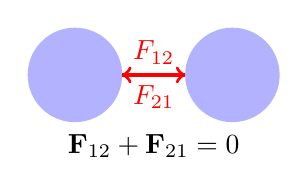
\begin{tikzpicture}
  \fill[blue!30] (-1,0) circle (0.6) node {$m_1$};
  \fill[blue!30] (1,0) circle (0.6) node {$m_2$};
  \draw[->,very thick,red] (-0.4,0) -- (0.4,0) node[midway,above] {$F_{12}$};
  \draw[->,very thick,red] (0.4,0) -- (-0.4,0) node[midway,below] {$F_{21}$};
  \node at (0,-0.9) {$\mathbf{F}_{12}+\mathbf{F}_{21}=0$};
\end{tikzpicture}
\end{center}

\section{万有引力定律}

\begin{lawbox}[万有引力]
\[
\mathbf{F} = -G\frac{m_1 m_2}{r^2}\,\hat{\mathbf{r}}
\]
\textbf{前提}：Einstein 场方程的弱场低速极限
\end{lawbox}

\begin{derivationbox}[从 GR 到 Newton]
  $G_{\mu\nu}=\frac{8\pi G}{c^4}T_{\mu\nu}$ 弱场/静态/低速 $\to \nabla^2\phi=4\pi G\rho \to \phi=-GM/r \to \mathbf{F}=-m\nabla\phi=-GmM\hat{\mathbf{r}}/r^2$。
\end{derivationbox}

\begin{center}
\begin{tikzpicture}[scale=1.1]
  \fill[yellow!40] (0,0) circle (1.2) node[black] {$M$};
  \fill[blue!20] (3,0.8) circle (0.25) node[black] {$m$};
  \draw[->,very thick,red] (3,0.8) -- (1.8,0.5);
  \draw[dashed,gray] (0,0) -- (3,0.8);
  \node at (1.5,0.2) {$r$};
  \draw[->,principleblue,thick] (3,1.5) arc (30:330:2.5 and 0.5);
  \node[principleblue] at (1,-1.0) {轨道};
  \node at (3,-1.5) {$F\propto\frac{1}{r^2}$——$D=3$ 的几何必然};
\end{tikzpicture}
\end{center}

\textbf{为什么是 $1/r^2$？} Gauss 定理在 $D$ 维空间中：场通量 $\propto r^{D-1}$。力 $\propto 1/r^{D-1}$。$D=3 \implies$ 力 $\propto 1/r^2$。如果 $D\neq 3$，就不存在稳定的行星轨道。

\section{Kepler 第三定律}

\begin{lawbox}[Kepler III]
\[
T^2 \propto r^3
\]
\end{lawbox}

\begin{derivationbox}[推导：圆形轨道近似]
  $mv^2/r = GMm/r^2 \implies v^2 = GM/r$。$T = 2\pi r/v \implies T^2 = (4\pi^2/GM)r^3$。
\end{derivationbox}

\begin{center}
\begin{tikzpicture}[scale=1.2]
  \draw (0,0) ellipse (2.5 and 0.8);
  \fill[yellow!40] (0.8,0) circle (0.4) node[black] {\tiny Sun};
  \fill[blue!20] (-2.1,0.3) circle (0.15);
  \draw[dashed] (0.8,0) -- (-2.1,0.3) node[midway,above] {$r$};
  \draw[->] (-2.1,0.6) arc (60:420:2.3 and 0.75);
  \node at (0,-1.5) {$T^2\propto r^3$（轨道周期的平方与半长轴的立方成正比）};
\end{tikzpicture}
\end{center}

\section{推导关系总图}

\begin{center}
\begin{tikzpicture}[
  node distance=1.2cm,
  kernel/.style={rectangle,draw,fill=principleblue!15,rounded corners,text width=2.2cm,align=center,font=\footnotesize\bfseries},
  law/.style={rectangle,draw,fill=lawgreen!15,rounded corners,text width=2.5cm,align=center,font=\footnotesize},
  arrow/.style={->,>=Stealth,thick,deriveorange}
]
  \node[kernel] (r2) {R2\\$\delta S = 0$};
  \node[kernel,right=0.5cm of r2] (r1) {R1\\时空};
  \node[law,below=0.6cm of r2] (el) {Euler-Lagrange};
  \node[law,below=0.4cm of el] (n2) {Newton II\\$F=ma$};
  \node[law,left=0.3cm of n2] (n1) {Newton I\\惯性};
  \node[law,right=0.3cm of n2] (n3) {Newton III\\$F_{12}=-F_{21}$};
  \node[law,below=0.4cm of n2] (gr) {万有引力\\$F=GmM/r^2$};
  \node[law,below=0.4cm of gr] (kep) {Kepler III\\$T^2\propto r^3$};
  \draw[arrow] (r2) -- (el); \draw[arrow] (el) -- (n1.west);
  \draw[arrow] (el) -- (n2); \draw[arrow] (r2) -- (n3.north);
  \draw[arrow] (r1) -- (gr); \draw[arrow] (n2) -- (gr);
  \draw[arrow] (gr) -- (kep);
\end{tikzpicture}
\end{center}

参考文献：[GOLD] Ch.1--2, [LAND] §1--3, [NEWTON], [NOETHER]
